\chapter{Detalles de implementación}\label{cap:implementation_details}
%Con el objetivo de ejemplificar las posibles aplicaciones del programa desarrollado se proponen un conjunto de aplicaciones del análisis causal en diversas áreas de la ciencia. Los modelos usados se basan en los propuestos en un conjunto de artículos académicos donde se emplea el anális causal para proponer soluciones a problemas relacionados con la medicina, la epidemiología y la psicología (\cite{matsuura2009structural, oh2001development, steiger2021causal}). Estos fueron simplificados y adaptados para satisfacer las restricciones del programa implementado. Todos los resultados mostrados en las siguientes secciones se corresponden con las salidas provistas por el programa.
%
%\section{Control de la COVID-19}
%
%La causalidad ha resultado ser especialmente útil en el área epidemiológica. Desde la aparición de la COVID-19 se han presentado trabajos donde se utiliza la inferencia causal para determinar qué factores disminuyen el riesgo de contagio y cuáles lo incrementan. \cite{bonvini2021causal, steiger2021causal}.
%
%Supongamos que se quiere poner en práctica un conjunto de medidas en una ciudad destinadas a frenar un brote de COVID-19. Dado que dichas medidas demandan recursos y no se conoce cuán efectivas serán, parece razonable utilizar una herramienta para estimar el resultado de su aplicación.
%
%Primeramente es necesario construir un modelo que declare explícitamente las relaciones de causalidad entre las variables de estudio. Este modelo puede obtenerse de dos maneras. La primera consiste en, utilizando un algoritmo, encontrar relaciones de causalidad subyacentes en los datos. Esta variante es conocida como \textit{descubrimiento causal}. La segunda vía consiste en construir el modelo a partir de un conjunto de presuposiciones producto de la experiencia o la intuición. Se optará por la segunda variante.
%
%\begin{figure}[h]
%	\centering
%	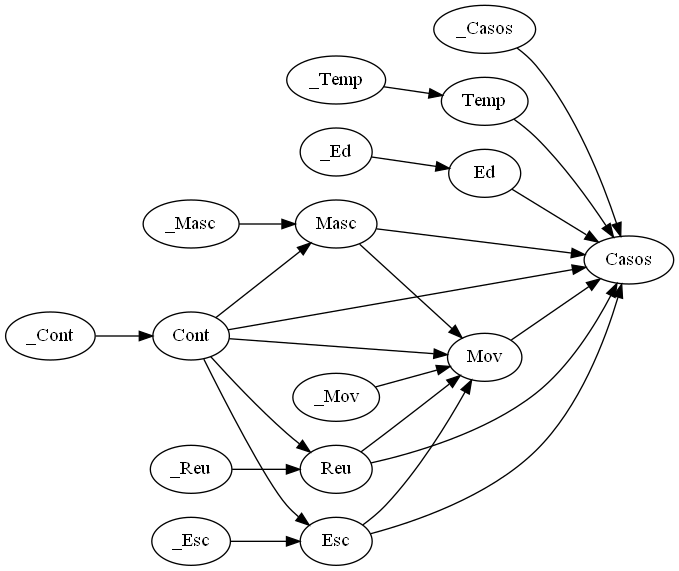
\includegraphics[width=\linewidth]{./images/Chapter-4/covid-graph}
%	\caption{Grafo causal asociado al modelo sobre la COVID-19}
%	\label{fig:covid-graph}
%\end{figure}
%
%En la Tabla \ref{tab:variables} se muestran las variables tenidas en cuenta para la construcción del modelo. Todas las variables toman valores numéricos. En los casos en que la variable sea binaria, el valor $1$ indica que la variable toma valor verdadero. En las variables categóricas, cada valor tiene asociado una categoría de la variable. Cada variable endógena tiene asociada un término de error o variable exógena cuyo nombre es el mismo pero con el prefijo \textquotedblleft\_\textquotedblright añadido. Estas variables no son incluidas en la tabla por simplicidad pero forman parte de la función de definición de las variables y añaden no-determinismo al modelo.
%\begin{table}
%	\begin{tabular}{| m{1.5cm} | m{2cm} | m{5cm}| m{3cm} |}
%		\hline
%		Nombre & Tipo & Valores & Descripción \\
%		\hline
%		Temp & Categórica & 0(baja), (1) media, (2) alta & Temperatura \\
%		\hline
%		Ed & Categórica & 0 (niño), 1(joven), 2(adulto), 3(anciano) & Edad \\
%		\hline
%		Gen & Categórica & 0(Hombre), 1(Mujer) & Género \\
%		\hline
%		DP & Categórica & 0(baja), 1(media), 2(alta) & Densidad de población \\
%		\hline
%		Cont & Categórica & 0(bajo), 1(medio), 2(alto) & Nivel de contagio \\
%		\hline
%		Masc & Binaria & 0,1 & Uso obligatorio de mascarilla \\
%		\hline
%		Reu & Binaria & 0,1 & Prohibición de reuniones masivas \\
%		\hline
%		Esc & Binaria & 0,1 & Cierre de las escuelas \\
%		\hline
%		Mov & Categórica & 0(bajo), 1(medio), 2(alto) & Nivel de movilidad \\
%		\hline
%		Casos & Categórica & pocos, normal, muchos & Número de casos reportados \\
%		\hline
%	\end{tabular}
%	\caption{Variables endógenas del modelo de la COVID-19}
%	\label{tab:variables}	
%\end{table}
%
%A partir de los datos extraídos se pueden obtener las marginales de las variables. La tabla \ref{tab:marginals} muestra la correspondiente al número de casos reportados. Como se observa existe una tendencia a diagnosticar un número alto de casos en la ciudad. Para contrarrestar este comportamiento se debe tomar un conjunto de medidas. Por ejemplo, establecer el uso obligatorio de mascarillas puede reducir el riesgo de brotes. El resultado de esta medida se puede calcular a partir de la intervención $P(Casos \mid do(Masc=1))$ y se muestra en la tabla \ref{tab:int}. Sin embargo, a pesar de que su aplicación disminuye el riesgo de un número alto de casos,  no es suficiente. En el caso de que se aplicase solo esta medida y el número de casos siga siendo alto, cabría preguntarse que hubiera ocurrido si además se hubiesen tomado medidas adicionales, como cerrar las escuelas, restringir la movilidad y prohibir las reuniones en masa. El contrafactual $P(Casos_{Masc=1, Esc=1, Reu=1, Mov=0} \mid Masc=1, Casos=2)$ da respuesta a esta interrogante y se muestra en la tabla \ref{tab:count}.
%
%\begin{table}[h!]
%	\centering
%	\begin{tabular}{| c | m{1.2cm} | m{1.2cm}| m{1.2cm} |}
%		\hline
%		v & pocos & normal & muchos \\
%		\hline
%		P(v) & 0.1372 & 0.2683 & 0.5945 \\
%		\hline
%	\end{tabular}
%	\caption{Marginal correspondiente a la variable Casos}
%	\label{tab:marginals}
%\end{table}
%
%\begin{table}[h!]
%	\centering
%	\begin{tabular}{| c | m{1cm} | m{1cm}| m{1cm} |}
%		\hline
%		v & bajo & medio & alto \\
%		\hline
%		P(v) & 0.196 & 0.3046 & 0.4994 \\
%		\hline
%	\end{tabular}
%	\caption{Marginal correspondiente a la variable Casos resultante de calcular la intervención $P(Casos \mid do(Masc=1))$}
%	\label{tab:int}
%\end{table}
%
%\begin{table}[h!]
%	\centering
%	\begin{tabular}{| c | m{1cm} | m{1cm}| m{1cm} |}
%		\hline
%		v & bajo & medio & alto \\
%		\hline
%		P(v) & 0.6432 & 0.1167 & 0.2402 \\
%		\hline
%	\end{tabular}
%	\caption{Marginal correspondiente a la variable Casos resultante de calcular el contrafactual $P(Y_{Masc=1, Esc=1, Reu=1, Mov=0} \mid Masc=1,Casos=2)$}
%	\label{tab:count}
%\end{table}
%
%\vspace{100px}
%\section{Comportamiento antisocial en adolescentes}
%Con el objetivo de entender el comportamiento antisocial en los adolescentes se estudian un conjunto de factores que se sospecha que pueden estar relacionados a este. Las variables tenidas en cuenta son: la autoestima del individuo (SE), situaciones adversas durante la niñez (ACE), síntomas de hiperactividad y déficit de atención (ADHD) y el nivel de agresividad en el individuo (AGR). Para medir el valor de cada variable en un individuo se le aplican una serie de tests, que devuelven una puntuación entre 0 y 4 para cada variable. Con estos datos, y con hipótesis a partir de estudios previos se construye un modelo cuyo diagrama corresponde al de la figura \ref{fig:agression}. A partir de los datos recopilados se determina la distribución que corresponde a los términos de error, así como la función que determina a cada variable.
%
%\begin{figure}[h!]
%	\centering
%	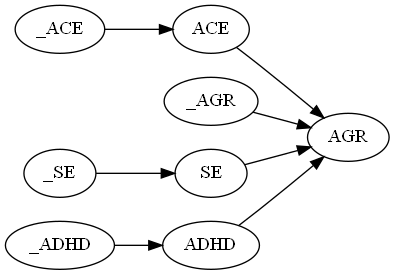
\includegraphics[width=.7\linewidth]{./images/Chapter-4/agression.png}
%	\caption{Grafo causal que explica el comportamiento agresivo en los adolescentes}
%	\label{fig:agression}
%\end{figure}
%
%\begin{figure}[h!]
%	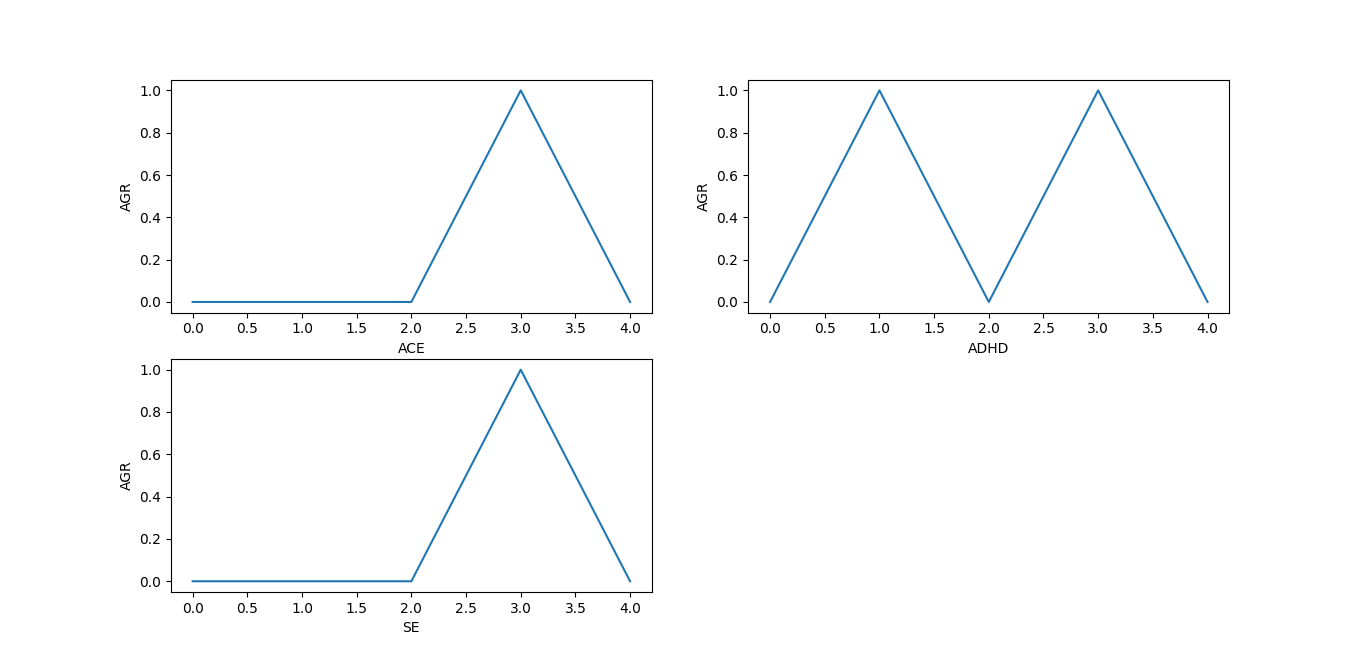
\includegraphics[width=\linewidth]{./images/Chapter-4/agression-charts.png}
%	\caption{Efecto total de las variables sobre el comportamiento agresivo del individuo}
%	\label{fig:agression-charts}
%\end{figure}
%
%Para determinar cuánto afecta cada variable al comportamiento del individuo se calcula el efecto total que ejerce cada variable sobre el comportamiento agresivo del individuo. En la figura \ref{fig:agression-charts} se muestra para cada variable $V$, por cada valor $v_i$, el efecto total $V$ sobre $AGR$ cuando $V$ cambia de $v_i$ hacia $v_{i+1}$. Como se puede observar, los valores extremos de las variables no aumentan el comportamiento agresivo del individuo y sí los intermedios.
%
%\section{Factores de riesgo de arteriosclerosis}
%Con el objetivo de aclarar las relaciones de causalidad entre los factores de riesgo de arteriosclerosis, se construye el modelo representado en la figura \ref{fig:arteriosclerosis}.
%Las variables de interés son edad(Ed), consumo de cigarro(Sm), alcohol(Al), realización de ejercicio físico(Ex), obesidad(Ob), hiperlipidemia(Lipid) e hipertensión(Hyper). Todas son binarias excepto la edad, que toma cuatro valores posibles: niño, joven, adulto y anciano.
%\begin{figure}[h!]
%	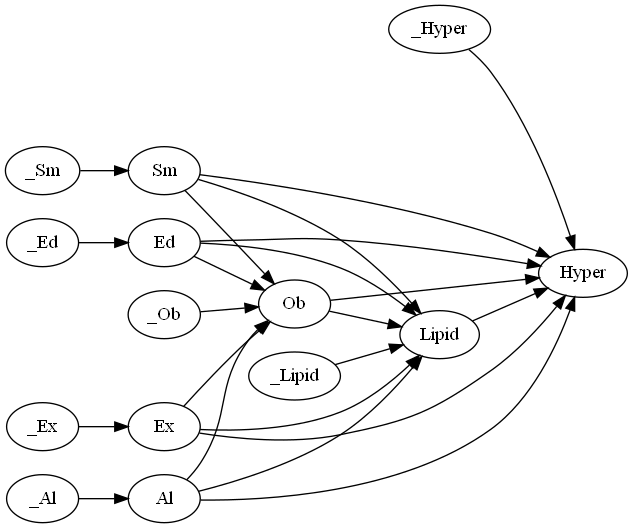
\includegraphics[width=\linewidth]{./images/Chapter-4/arteriosclerosis.png}
%	\caption{Grafo causal correspondiente al modelo que explica los factores de riesgo de arteriosclerosis.}
%	\label{fig:arteriosclerosis}
%\end{figure}
%
%Los valores que toman las marginales de las variables de obesidad, hiperlipidemia e hipertensión a partir de los datos recogidos y sin realizar ninguna observación sobre el modelo se recogen en la tabla \ref{table:art-non-evidence}.
%
%\vspace*{20px}
%
%\begin{table}
%	\centering
%	\begin{tabular}{| m{1cm} | m{1cm} | m{1cm}|}
%		\hline
%		V & P(V=0) & P(V=1)\\
%		\hline
%		Ob & 0.574 & 0.426 \\			
%		\hline
%		Lipid & 0.664 & 0.336 \\
%		\hline
%		Hyper & 0.5092 & 0.4908 \\
%		\hline
%	\end{tabular}
%	\caption{Marginales correspondientes a las variables Ob(Obesidad), Hyper(Hipertensión) y Lipid(Hiperlipidemia), obtenidas a partir de los datos recopilados}
%	\label{table:art-non-evidence}
%\end{table}
%
%Alternativamente al efecto total, se puede utilizar la fórmula del \textit{Efecto Causal Promedio}(ACE):
%	\[ ACE = P(Y=1 \mid do(X=1)) - P(Y=1 \mid do(X=0)) \]
%El Efecto Causal Promedio se aplica entre dos variables binarias y compara el porciento de individuos que responden positivamente a un tratamiento con los que lo hacen si no se les aplica dicho tratamiento. Permite medir en términos de probabilidades cuánto influye una variable en otra. En dependencia del signo del resultado, se determina si este efecto es positivo o negativo y su módulo nos dice cuán relevante es este efecto. En la tabla \ref{table:ace} se muestra el valor de ACE entre cada una de las variables de Hipertensión, Hiperlipidemia y Obesidad y las variables de Ejercicio, Alcohol y Fumar. Como se puede apreciar, el consumo de cigarro y alcohol incrementa el riesgo de contraer Hipertensión, Hiperlipidemia y Obesidad mientras que la práctica de ejercicio físico lo disminuye.
%
%\begin{table}[h!]
%	\centering
%	\begin{tabular}{| m{1.2cm} | m{1.2cm} | m{1.2cm}| m{1.2cm} |}
%		\hline
%		& Ob & Lipid & Hyper \\
%		\hline
%		Al & 0.524 & 0.3872 & 0.4952 \\			
%		\hline
%		Sm & 0.365 & 0.32 & 0.422 \\
%		\hline
%		Ex & -0.115 & -0.265 & -0.172 \\
%		\hline
%	\end{tabular}
%	\caption{Efecto Causal Promedio (ACE) que ejercen las variables Al, SM y Ex sobre los factores de riesgo.}
%	\label{table:ace}
%\end{table}
%
%Por último, aprovechando que la mayoría de las variables son binarias, se puede realizar un análisis de atribución para determinar cuán necesarias y suficientes son las variables causa (Al, Ex, Sm) para determinar los valores de las variables efecto (Ob, Hyper, Lipid). En las tablas \ref{table:attr-Al} y \ref{table:attr-Sm} se muestran los valores de PN(probabilidad de necesidad), PS(probabilidad de suficiencia) y PNS(probabilidad de necesidad y suficiencia) para las causas Al y Sm respectivamente. En el caso de la variable $Ex$, todas las probabilidades tienen valor cero, lo cual tiene sentido teniendo en cuenta que el ACE dio negativo en todos los casos. Esto significa que la práctica de ejercicio físico no nos permite afirmar que existirán factores de riesgo y que la existencia de factores de riesgo no implica que el individuo realice ejercicio físico. 
%
%\begin{table}[h!]
%	\centering
%	\begin{tabular}{| m{1.2cm} | m{1.2cm} | m{1.2cm}| m{1.2cm} |}
%		\hline
%		& PN & PS & PNS \\
%		\hline
%		Ob & 0.7616 &  0.6268 & 0.5240 \\			
%		\hline
%		Lipid & 0.7311 & 0.4515 & 0.3872 \\
%		\hline
%		Hyper & 0.6706 & 0.6543 & 0.4952 \\
%		\hline
%	\end{tabular}
%	\caption{Análisis de atribución sobre la variable Al}
%	\label{table:attr-Al}
%\end{table}
%
%\begin{table}[h!]
%	\centering
%	\begin{tabular}{| m{1.2cm} | m{1.2cm} | m{1.2cm}| m{1.2cm} |}
%		\hline
%		& PN & PS & PNS \\
%		\hline
%		Ob & 0.5659 &  0.5069 & 0.3650 \\			
%		\hline
%		Lipid & 0.6061 & 0.404 & 0.3200 \\
%		\hline
%		Hyper & 0.5672 & 0.6224 & 0.4220 \\
%		\hline
%	\end{tabular}
%	\caption{Análisis de atribución sobre la variable Sm}
%	\label{table:attr-Sm}
%\end{table}






